\documentclass[titlepage]{article}

\usepackage[utf8]{inputenc}
\usepackage[english]{babel}
\usepackage[IL2]{fontenc}
\usepackage{graphicx}
\usepackage{syntax}

%\usepackage{mathtools}

\title{Compiler construction - VYPe15 project documentation}
\author{
	Kidoň Marek\\
	\texttt{xkidon00@stud.fit.vutbr.cz}
\and
	Janošík, Ondřej\\
	\texttt{xjanos12@stud.fit.vutbr.cz}
}
\date{}


\begin{document}
\maketitle

\section{Introduction}
This paper describes the architecture and implementation of the \textit{VYPe15} language
compiler. The compiler itself is implemented in Haskell without any use of compiler
automation
tools such as \textbf{lex} \cite{lex}, \textbf{yacc} \cite{yacc} or
other tools for reasons that will be explained in chapter
\ref{sec:implementation}. Also the well established concept of
syntax directed translation was slightly violated.
We will explain why in chapter \ref{sec:architecture}.

\section{Architecture}
\label{sec:architecture}

\subsection{High-level architecture}
In the figure \ref{fig:architecture}, we can see the high-level architecture of our
compiler. As you can see we violated concept of syntax-directed translation.

\begin{figure}[h!]
	\centering
	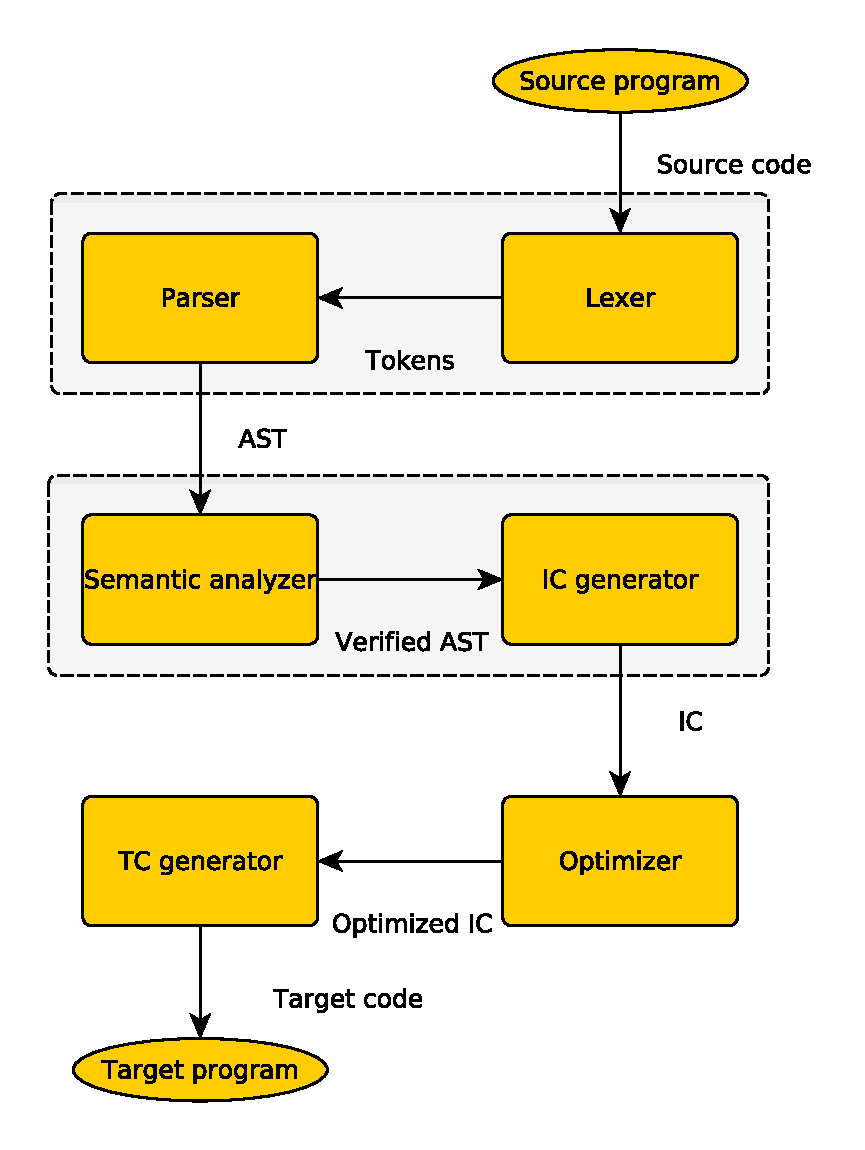
\includegraphics[scale=0.5]{figures/compilerArchitecture}
	\caption{High-level architecture of our compiler.}
	\label{fig:architecture}
\end{figure}

We omitted the semantic analyzer from the syntax analyzer an left it with the intermediate
code generator as a standalone component instead. Numerous reasons lead is to this decision
such as :

\begin{itemize}
	\item the monadic parser stack would be way too complex to produce reasonable code
		(see chapter \ref{sec:implementation} for further information),
	\item Haskell is lazy-evaluated, so putting semantic analyzer behind the parser does
		not necessarily mean that semantic analysis is performed \textit{after}
		parsing is done.
\end{itemize}

The last two components are the optimizer and target code generator duo, which is fairly
standard.

\subsection{Grammar}
In our parser we implemented the following grammar.

\begin{verbatim}
<program> : ( <funcDeclr> | <funcDef> )*
<funcDeclr> : (<dataType> | 'void') <identifier> '(' <typeParamList> ')' ';'
<funcDef> : (<dataType> | 'void') <identifier> '(' <paramList> ')' (<statement>)*
<dataType> : ('int' | 'char' | 'string')
<typeParamList> : 'void'
                | <dataType> (, <dataType>)*
<paramList> : 'void'
            | <dataType> <identifier> (, <dataType> <identifier>)*
<statement> : <identifier> = <expression> ';'
            | 'while' '(' <expression> ')' '{' (<statement>)* '}'
            | 'if' '(' <expression> ')' '{' (<statement>)* '}'
              'else' '{' (<statement>)* '}'
            | 'return' ( <expression> ';' | ';' )
            | <identifier> '(' ')' ';'
            | <identifier> '(' <expression> (',' <expression>)* ')' ';'
            | <dataType> <identifier> {',' <identifier>} ';'
<expression> : <expression> ( '||' | '&&' | '==' | '!=' | '<' | '>' | '<=' ) <expression>
             | <expression> ( '%' | '+' | '-' | '!' | '>=' | '*' | '/' ) <expression>
             | '('<dataType>')'
             | <identifier>
             | <identifier> '(' ')' ';'
             | <identifier> '(' <expression> (, <expression>)* ')' ';'
             | <charLit>
             | <stringLit>
             | <numLit>
\end{verbatim}

Please note that comments and other lexer related parts of grammar are not displayed.
The \texttt{<identifier>}, \texttt{<charLit>}, \texttt{<stringLit>} and \texttt{<numLit>}
production rules are taken directly from project assignment, so we don't specify them
again. Because this grammar can't be implemented using the standard LL(1) parser, we
used higher order LL grammar as described in section \ref{sec:implementation}.

\section{Implementation}
\label{sec:implementation}

\subsection{Semantic analyzer}
Our parser was implemented using Haskell's \texttt{Parsec}
\footnote{https://hackage.haskell.org/package/parsec} library. It is
an industrial-grade monadic parser library for LL(*) parser implementation. Parsers
implemented using the Parsec library are fast, deliver very good error messages and
are generic on the input stream type.

The expression parser was generated using parser generator delivered as a part of the
library. The rest of the parser has been however implemented manually. It seems like an
unnecessary work, but since Parsec supports applicative-style programming,
constructing the parser is very similar to writing the actual grammar thanks to the well
designed combinators such as the \texttt{many}, \texttt{<|>} and others.

We are very satisfied with the way our solution works compare to the \texttt{happy}
\footnote{https://www.haskell.org/happy/} \cite{happy} and \texttt{alex}
\footnote{https://www.haskell.org/alex/} solution we used in early stages. The number one
reason is that the parser description in the happy language is not part of our
compiler, which makes the debugging process much more time consuming and difficult
because there is no type safety. Although happy would generate a parser, the parser
might not be correct. This won't happen in Parsec since the parser description is
part of our compiler program.
On the other hand the happy generated parser is exceptionally fast (Haskell compiler
itself uses the happy compiler generator), but its error reporting is worse than in
case of Parsec \footnote{in general, parsing in haskell is usually a trade-of between performance
and error massage reporting}.

\subsection{Semantic analysis and code generation}
Semantic analysis works on the abstract syntax tree. It is a recursive algorithm that
utilizes the power of monads to handle tree traversal and semantic analysis while
simultaneously generating intermediate code. We constructed a monad stack consisting of
\texttt{ExceptT} for error handling and \texttt{Writer} for intermediate code instruction
storage.

\subsection{Optimization and code generation}
Unfortunately target code generation is performed directly from intermediate code because
we didn't find the time to implement it properly. Target code generation is implemented
using the \texttt{WriterT} and \texttt{State} monad stack. Writer serves as target code
instructions storage and State holds the register table plus some other information and
helps with simulating the stack frame in assembly language.

\section{Compilation}
\label{sec:compilation}
To compile this project the Haskell platform \footnote{https://www.haskell.org/platform/}
\footnote{tested on the \texttt{7.10.3 version}}
is required. It contains all necessary libraries for any serious haskell programming
and is de-facto a standard platform for Haskell developers. It contains the \texttt{GHC}
(Glorious Glasgow
Haskell compiler), some widely-used libraries and the \texttt{cabal} build system.
To compile our project just type \texttt{make}.

We use cabal to build our project so if cabal is missing, the project won't build.
All libraries used in our project are part of the Haskell platform.

\section{Conclusion}
In our project we implemented compiler for the VYPe15 programming language. Compiler
is written in Haskell, purely functional programming language. In chapter
\ref{fig:architecture} we explained that our compiler high-level design comes from the
fact
that Haskell is lazy evaluated and in chapter \ref{sec:implementation} we described the
implementation process and decisions we have taken.

We did not generate an LR parser (although we did so in early stages), instead we
implemented an LL(*) parser mainly for type safety reasons. The semantic analysis is
perform on an AST instead of being done directly alongside parsing. The semantic analyzer
and intermediate code generator are strongly connected in our project.

Optimizer for time reasons was not implemented and it is basically an identity
function in the end.

The section \ref{sec:compilation} describes necessary steps that are mandatory in order
to successfully compile our project.

\newpage
\bibliographystyle{alpha}
\bibliography{bibliography}
\end{document}
